%=================================================================
%CAPITULO III
%==================================================================

\chapter{Espacios separables, funciones continuas y subespacios}

La propiedad de los n\'umeros racionales, de ser densos dentro de
los n\'umeros reales, es de suma importancia. Esta situaci\'on es
planteada dentro de un e.m. con el concepto de separabilidad.
Asimismo veremos que sobre un e.m. tenemos la noci\'on de
funci\'on continua, definiremos este concepto y demostraremos
algunas propiedades b\'asicas. Tambi\'en veremos que una
m\'etrica, sobre determinado conjunto, induce una m\'etrica sobre
un subconjunto de \'el.

\section{Subespacios de un espacio m\'etrico}

Sea $(X,d)$ un e.m. e $Y\subset X$. La m\'etrica $d$ es una
funci\'on definida sobre $X\times X$, luego podemos considerar su
restricci\'on a $Y\times Y$. Esta restricci\'on tambi\'en
cumplir\'a, es inmediato verlo,  los axiomas de una m\'etrica. Por
este motivo, el par $(Y,d)$ es un e.m., por una abuso de
notaci\'on denotaremos la restricci\'on de $d$ al conjunto
$Y\times Y$ por el mismo s\'{\i}mbolo $d$.  Diremos que $Y$ es un
subespacio de $X$.  Observar que la forma de las bolas en un
subespacio puede ser diferente que en el espacio total, como puede
verse en la figura \vref{fig,bolasub}. En este gr\'afico $X$ es el
espacio ``total'', $Y$ el subespacio y $x$ es un punto sobre la
frontera de $Y$, entonces la bola en $Y$ de centro $x$ y radio $r$
es la parte que quedo cuadriculada en el dibujo. Pongamos
$B_Y(x,r)$ para la bola en $Y$ de centro  $x$ y radio $r$,
entonces tenemos la relaci\'on:

\begin{equation}\label{eq,bolasub}
    B_Y(x,r):=\{y\in Y: d(x,y)<r\}=B(x,r)\cap Y,
\end{equation}
donde $B(x,r)$ es la bola en el espacio total.
\begin{figure}[h]
\begin{center}
    \psfrag{total}{$X$}
    \psfrag{Y}{$Y$}
    \psfrag{x}{$x$}
    \psfrag{r}{$r$}
    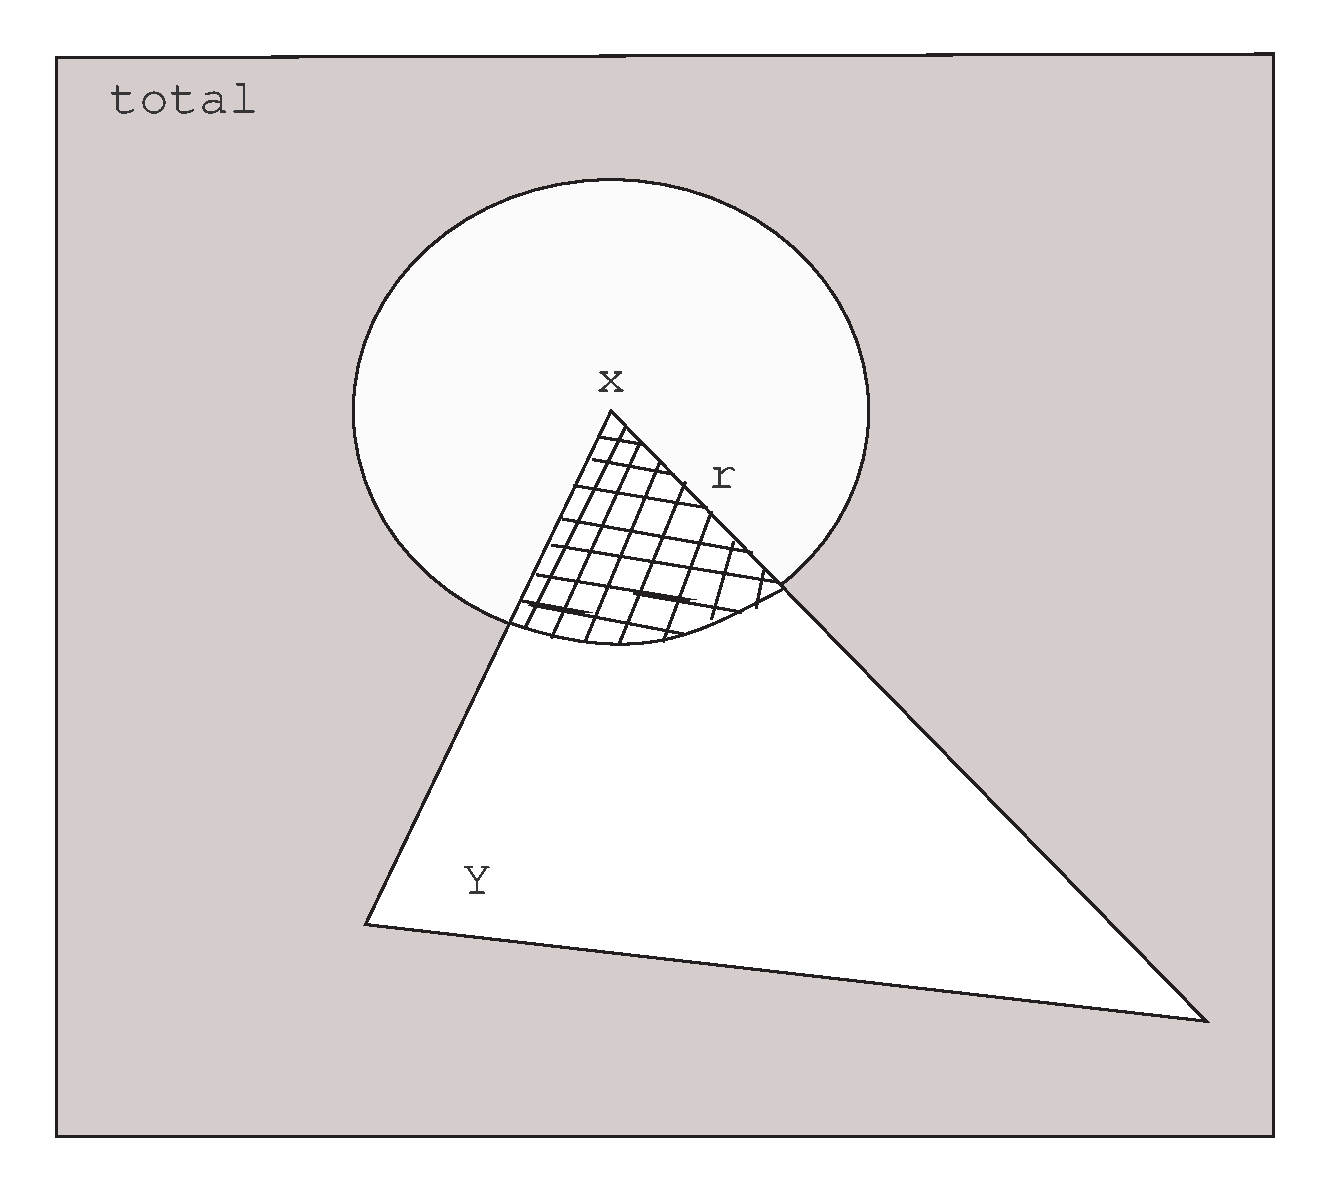
\includegraphics[height=9cm, width=10cm]{bolasub.eps}
    \caption{Una bola en un subepsacio}\label{fig,bolasub}
\end{center}
\end{figure}


El siguiente teorema nos d\'a una relaci\'on de los abiertos y
cerrados en $Y$ con los abiertos y cerrados en $X$.

\begin{teorema} Sea $(X,d)$ un e.m. e $Y\subset X$. Entonces:
\begin{itemize}
\item[a)] El conjunto $A$ es abierto en $Y$ si y solo si existe un
$G$ abierto en $X$ tal que $A=G\cap Y$.
\item[b)] El conjunto $C$ es cerrado en $Y$ si y solo si existe un
cerrado $F$ en $X$ tal que $C=Y\cap F$.
\end{itemize}
\end{teorema}
\begin{demo} Veamos, primero, la propiedad a). Sea $A$ un abierto
en $Y$. Para cada $x\in A$ existe, de acuerdo a la Ecuaci\'on
\vref{eq,bolasub}, un radio $r_x>0$ tal que:
\begin{equation}\label{eq,inclusiondebolas}
    B(x,r_x)\cap Y\subset A.
\end{equation}
Definamos:
\[
    G:=\bigcup\limits_{x\in A}B(x,r_x).
\]
El conjunto $G$ es abierto, pues la uni\'on de conjuntos abiertos
resulta abierto. Adem\'as
\[
    G\cap Y=\bigcup\limits_{x\in A}B(x,r_x)\cap Y= A.
\]
La \'ultima igualdad es cierta por la ecuaci\'on
\vref{eq,inclusiondebolas} y por que cada $x\in A$ est\'a en el
conjunto $B(x,r_x)\cap Y$. De modo que, encontramos el conjunto
que cumple la propiedad a).

Ahora la demostraci\'on de b) es sencilla de obtener. Sea $C$
cerrado en $Y$, en particular $C\subset Y$, entonces $Y-C$ es
abierto en $Y$. Por a) existe un abierto $G$ tal que:
\[
    Y-C=G\cap Y.
\]
Entonces
\[C=Y\cap G^c.\]
Como el conjunto $G^c$ es cerrado, obtenemos la tesis con $F=G^c$.
\end{demo}

\begin{proposicion}\label{pro,entornosub}Sea $(X,d)$ un e.m. e $Y\subset X$ un
subespacio. El conjunto $U\subset Y$ es un entorno de $x\in Y$ en
el espacio $(Y,d)$ si y solo si existe un entorno $V$ de $x$ en el
e.m. $(X,d)$ tal que $U=V\cap Y$.
\end{proposicion}
\begin{demo} Si $U$ es un entorno de $x$ en $Y$, entonces $x$
est\'a en el interior de $U$ relativo a $Y$ (pongamos $U^0_Y$ para
este conjunto). Como $U^0_Y$ es un abierto en $Y$, por el teorema
anterior, existe un abierto $W$ tal que $U^0_Y=Y\cap W$. Tomemos
$V=W\cup U$. El conjunto $V$ es un entorno de $x$ en $(X,d)$, pues
contiene al conjunto $W$ que lo es. Adem\'as $V\cap Y=U$, lo que
demuestra la aserci\'on.
\end{demo}

\begin{figure}[h]
\begin{center}
    \psfrag{X}{$X$}
    \psfrag{Y}{$Y$}
    \psfrag{x}{$x$}
    \psfrag{U}{$U$}
    \psfrag{W}{$W$}
    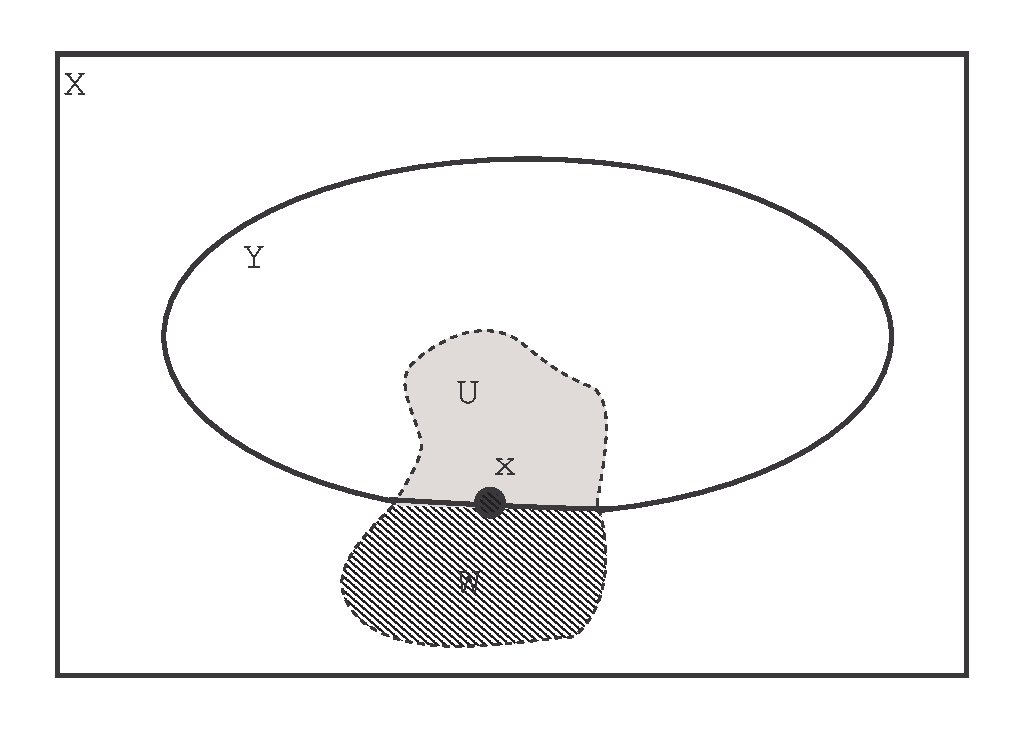
\includegraphics[height=6cm, width=10cm]{entosub.eps}
    \caption{Demostraci\'on de la Proposici\'on
    \ref{pro,entornosub}}\label{fig,entosub}
\end{center}
\end{figure}





\begin{proposicion} Sea $(X,d)$ un e.m. e $Y\subset X$ un
subespacio. Supongamos que $A\subset Y$. Entonces la clausura de
$A$ en el subespacio $Y$ (denotemos esto por $\overline{A}^Y$) es
igual a $\overline{A}^Y=\overline{A}\cap Y$.
\end{proposicion}
\begin{demo} El conjunto $\overline{A}\cap Y$ es un cerrado en $Y$
que contiene al conjunto $A$, de modo que
$\overline{A}^Y\subset\overline{A}\cap Y$. Veamos la otra
inclusi\'on. Sea $x\in \overline{A}\cap Y$. Como $x\in
\overline{A}$ entonces para todo entorno $U$ de $x$, tenemos que
$U\cap A\neq\emptyset$. Como $A\subset Y$ tenemos que $(U\cap
Y)\cap A=U\cap A\neq\emptyset$. As\'{\i}, como $U\cap Y$ es un
entorno  arbitrario de $X$ en el subespacio $Y$, tenemos que
$x\in\overline{A}^Y$.
\end{demo}
\section{Espacios separables}
\begin{definicion} Sea $(X,d)$ un e.m.. Un conjunto $A\subset X$
se dir\'a \emph{denso en }$B\subset X$ si $\overline{A}\supset B$.
Si el conjunto $A$ es denso en $X$ se dir\'a, brevemente, que $A$
\emph{es denso}.
\end{definicion}
\begin{ejemplo} $\mathbb{R}-\{0\}$, $\mathbb{Q}$ son densos en $\mathbb{R}$.
\end{ejemplo}
\begin{ejemplo} Sea $(X,d)$ un e.m discreto. Entonces $A$ es denso
si y solo si $A=X$. En efecto, tenemos que $\overline{A}=X$, de
modo que si $x\in X$  todo entorno de $x$ interseca al conjunto
$A$. De modo que  $B(x,1/2)\cap A\neq\emptyset$. Pero, como se
sabe, $B(x,1/2)=\{x\}$, de modo que $x\in A$. Esto demuestra que
$X=A$.
\end{ejemplo}

\begin{definicion} Un e.m. $(X,d)$ se dir\'a separable si tiene un
subconjunto denso y a lo sumo numerable.
\end{definicion}

\begin{ejemplo} Como se dijo $\mathbb{Q}$ es un conjunto denso,
adem\'as es numerable, por consiguiente $\mathbb{R}$ es separable.
\end{ejemplo}

\begin{ejemplo}\label{ej,rndenso} $\mathbb{R}^n$ con la m\'etrica euclidea es
separable. Afirmamos que $\mathbb{Q}^n$ es un conjunto denso y
numerable. Para verlo, tomemos $x=(x_1,...,x_n)\in \mathbb{R}^n$ y
veamos que est\'a en $\overline{\mathbb{Q}^n}$. Para ello es
suficiente probar que $B(x,r)\cap \mathbb{Q}^n\neq\emptyset$, para
todo $r>0$. Sea $r>0$ un radio, no es muy dificil demostrar, ver
la figura \vref{fig,rndenso}, la siguiente inclusi\'on de un
``cubo'' en la bola:
\[
    (x_1-\frac{r}{\sqrt{n}},x_1+\frac{r}{\sqrt{n}})\times\dots\times
    (x_n-\frac{r}{\sqrt{n}},x_n+\frac{r}{\sqrt{n}})\subset B(x,r).
\]
Como $\mathbb{Q}$ es denso en $\mathbb{R}$ existen racionales
$q_i\in (x_i-\frac{r}{\sqrt{n}},x_i+\frac{r}{\sqrt{n}})$,
$i=1,...,n$. En virtud de esto $(q_1,...,q_n)\in\mathbb{Q}^n\cap
B(x,r)$. Y as\'{\i} queda establecida la afirmaci\'on.

\begin{figure}[h]
\begin{center}
    \psfrag{x}{$x$}
    \psfrag{y}{$y$}
    \psfrag{x1}{$x-\frac{r}{\sqrt{2}}$}
    \psfrag{x2}{$x+\frac{r}{\sqrt{2}}$}
    \psfrag{y1}{$y-\frac{r}{\sqrt{2}}$}
    \psfrag{y2}{$y+\frac{r}{\sqrt{2}}$}
    \psfrag{q1}{$q_1$}
    \psfrag{q2}{$q_2$}
    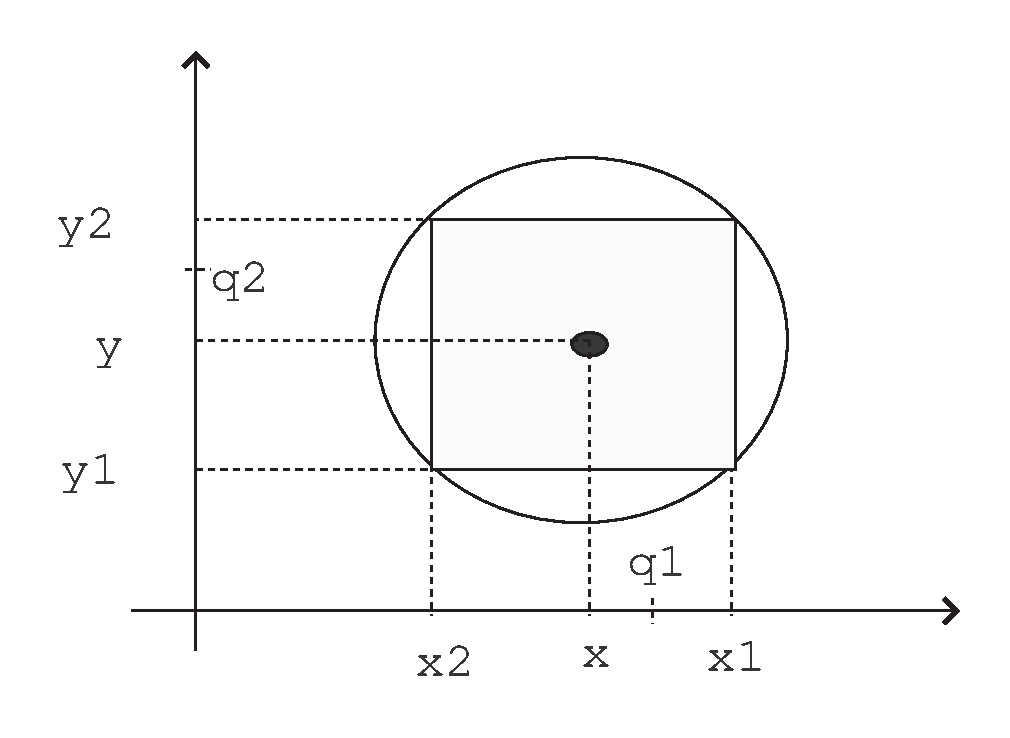
\includegraphics[height=7.5cm, width=10cm]{rndenso.eps}
    \caption{Construcci\'on del Ejemplo
    \ref{ej,rndenso}}\label{fig,rndenso}
\end{center}
\end{figure}
\end{ejemplo}

\begin{ejemplo} Un e.m. discreto $(X,d)$ es separable si y solo si
$X$ es a lo sumo numerable. Como vimos en un ejemplo anterior el
\'unico conjunto denso que hay en un e.m. discreto es el total, de
modo que si el espacio es separable $X$ debe ser a lo sumo
numerable.
\end{ejemplo}

\begin{definicion} En un e.m. $(X,d)$, una familia de conjuntos
abiertos $\{G_i\}_{i\in I}$ se dir\'a \emph{base} si todo abierto
se puede obtener como uni\'on de miembros de la familia. M\'as
precisamente, si $G$ es un abierto cualquiera existe un
subconjunto de sub\'{\i}ndices $J\subset I$ tal que:
\[
    G=\bigcup_{i\in J}G_i.
\]
\end{definicion}

\begin{ejemplo} En cualquier e.m. $(X,d)$ la familia de todas las
bolas es una base. Tambi\'en es una base la familia de todas las
bolas con radio igual a $1/n$ con $n\in \nn$. En efecto, si $G$ es
un abierto cualquiera, para todo $x\in G$ existe un $r_x>0$ tal
que $B(x,r_x)\subset G$. As\'{\i} podemos ver que
\[
    G=\bigcup\limits_{x\in G}B(x,r_x),
\]
lo que demuestra que $G$ lo podemos escribir como uni\'on de
bolas. Para el otro caso elegimos un natural $n_x$ suficientemente
grande para que $1/n_x<r_x$.
\end{ejemplo}

\begin{proposicion}\label{pro,caracbase} Una familia de abiertos $\{G_i\}_{i\in I}$ es
una base si y solo si para todo $x\in X$ y para todo entorno $U\in
E(x)$, existe un $i\in I$ tal que:
\[
    x\in G_i\subset U.
\]
\end{proposicion}
\begin{demo} $\Rightarrow )$. Sea $x\in X$ y $U\in E(x)$. Como la familia es
base, tenemos que $U^0$ es uni\'on de miembros de la familia.
Adem\'as, por definici\'on, tenemos que $x\in U^0$, estos dos
hechos implican la tesis.

$\Leftarrow)$ Sea $G$ un abierto. Por hip\'otesis, para cada $x\in
G$ encontramos un $i_x\in I$ tal que $x\in G_{i_x}\subset G$.
As\'{\i} tenemos que:
\[
    G=\bigcup\limits_{x\in G}G_{i_x}.
\]
\end{demo}

\begin{teorema}\label{teo,basenum} Un e.m. es separable si y solo si existe una base
a lo sumo numerable.
\end{teorema}
\begin{demo}$\Leftarrow )$. Sea $\{G_n\}_{n\in\nn}$ una base numerable de
abiertos (si hubiera una base finita el razonamiento es
id\'entico). Elijamos $a_n\in G_n$. El conjunto
$D:=\{a_n:n\in\nn\}$ es, entonces, a lo sumo numerable (?` Por
qu\'e?). Adem\'as, veamos que es denso. Efectivamente, sea $x\in
X$ un punto arbitrario y $U\in E(x)$. Como consecuencia de la
Proposici\'on \vref{pro,caracbase} existe un $n\in\nn$ tal que
$x\in G_n\subset U$. Ahora tenemos el punto $a_n\in G_n$, y por
ello $U\cap D\neq\emptyset$. Probamos as\'{\i} que todo entorno de
$x$ interseca a $D$, en consecuencia $x\in \overline{D}$. Como el
$x$ es arbitrario, aquello prueba que $D$ es un conjunto denso.

$\Rightarrow )$. Sea $D$ un conjunto denso y a lo sumo numerable.
Definamos la siguiente familia de bolas abiertas:
\[
   \mathcal{A}:= \{B(x,\frac1n):x\in D \wedge n\in\nn\}.
\]
Esta es una familia a lo sumo numerable, pues la siguiente
funci\'on

\begin{eqnarray}
    T:\nn\times D&\longrightarrow\mathcal{A}\nonumber \\
    (n,x)&\longmapsto B(x,\frac1n)\nonumber \\
\end{eqnarray}
es suryectiva.

Veamos que la familia propuesta es una base de abiertos usando la
Proposici\'on \vref{pro,caracbase}. Sea $x\in X$ y $U\in E(x)$.
Como $x\in U^0$, podemos elejir $r>0$ tal que $B(x,r)\subset U$.
Sea, ahora, $n\in\nn$ suficientemente grande, de modo que $2/n<r$.
Como $D$ es denso debe existir un $a\in D$ tal que $a\in
B(x,\frac1n)$. Observes\'e que tenemos que $x\in B(a,1/n)$, ver
Figura \ref{fig,basenum}. Adem\'as, tenemos que $B(a,1/n)\subset
B(x,r)\subset U$. Para demostrarlo, tomemos $y\in B(a,1/n)$.
Entonces
\[
    d(x,y)\leq d(x,a)+d(a,y)<\frac1n+\frac1n=\frac2n<r.
\]
Tenemos as\'{\i} que $x\in B(a,1/n)\subset U$, como $B(a,1/n)$ es
un elemento de la familia propuesta, tenemos probada la propiedad
de la Proposicion \vref{pro,caracbase} y, de este modo, la familia
propuesta resulta una base.
\end{demo}
\begin{figure}
\begin{center}
    \psfrag{U}{$U$}
    \psfrag{x}{$x$}
    \psfrag{a}{$a$}
    \psfrag{1n}{$1/n$}
    \psfrag{r}{$r$}
    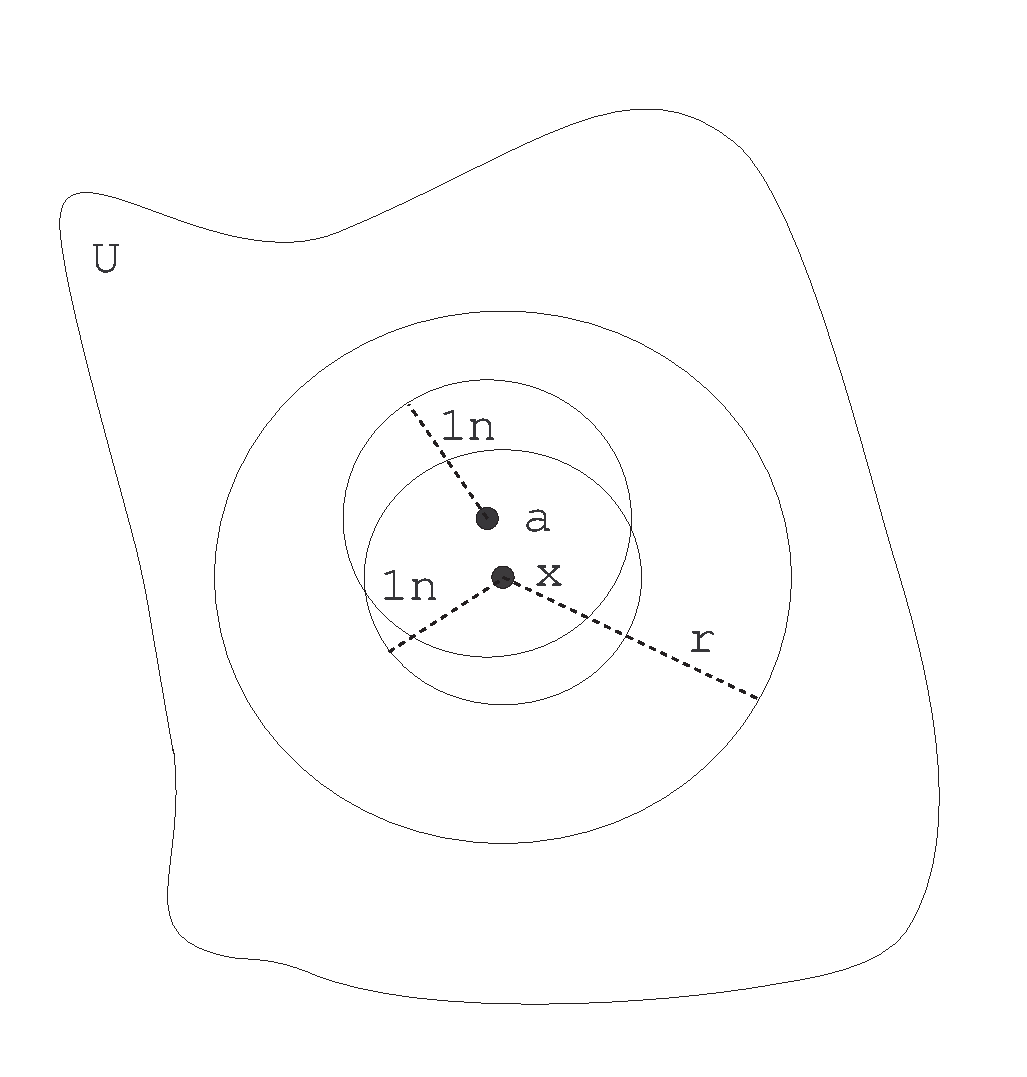
\includegraphics[height=8cm, width=8cm]{basenum.eps}
    \caption{Demostraci\'on del Teorema
    \ref{teo,basenum}}\label{fig,basenum}
\end{center}
\end{figure}
\begin{corolario} Un subespacio de un espacio separable es
separable.
\end{corolario}
\begin{demo} Sea $(X,d)$ un e.m. e $Y\subset X$. Sea $\{G_n\}_{n\in I}$
una base a lo sumo numerable de abiertos. Es f\'acil demostrar que
la familia $\{G_n\cap Y\}_{n\in I}$ es una base de los abiertos de
$Y$.
\end{demo}

\section{Funciones Continuas}
Vamos a ver que, en el contexto de los espacios m\'etricos,
podemos definir el concepto de que una funci\'on sea continua.

\begin{definicion} Sean $(X,d)$, $(Y,d')$ dos e.m, $f:X\rightarrow
Y$ una funci\'on y $x\in X$. Diremos que $f$ \emph{es continua en}
$x$ si para todo entorno  $V\in E(f(x))$, existe un entorno de
$U\in E(x)$ tal que $f(U)\subset V$ (ver Figura
\vref{fig,funccon}). Diremos que $f:X\rightarrow Y$ es
\emph{continua} si es continua en cada punto de $X$.
\end{definicion}

\begin{figure}
\begin{center}
    \psfrag{X}{$X$}
    \psfrag{Y}{$Y$}
    \psfrag{U}{$U$}
    \psfrag{V}{$V$}
    \psfrag{x}{$x$}
    \psfrag{y}{$f(x)$}
    \psfrag{f}{$f$}
    \psfrag{fU}{$f(U)$}
    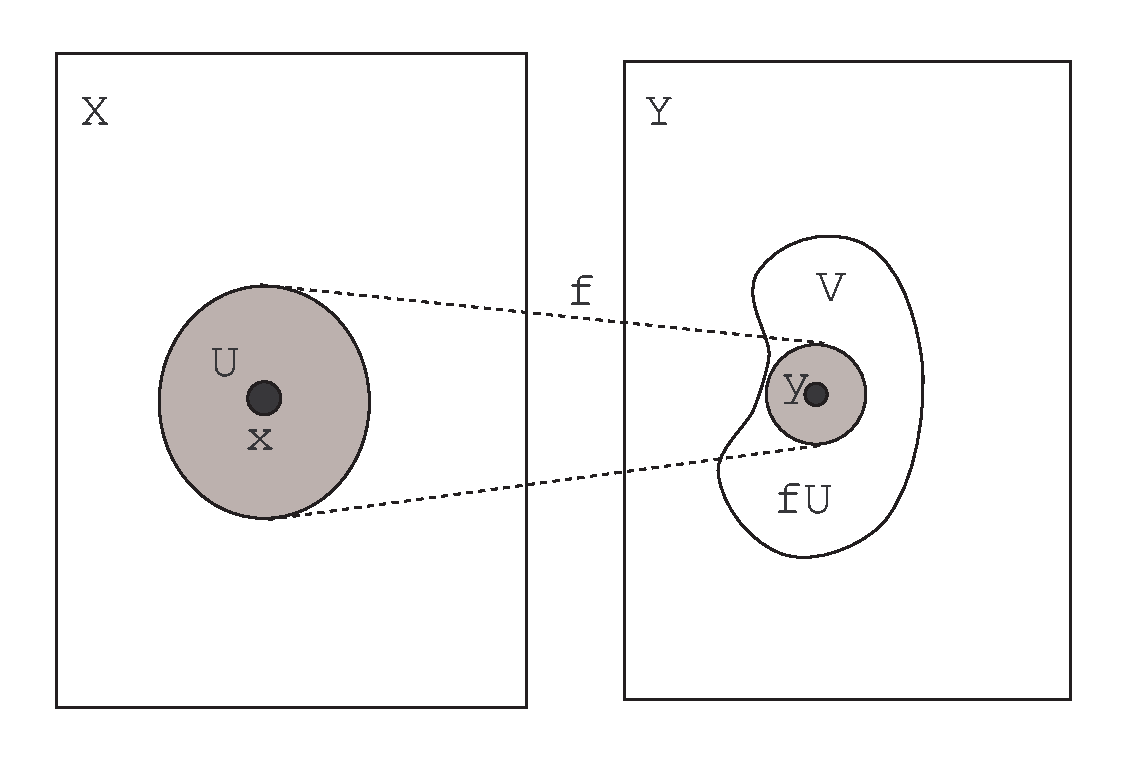
\includegraphics[height=7cm, width=9cm]{funccon.eps}
    \caption{Denfinici\'on de funci\'on
    continua}\label{fig,funccon}
\end{center}
\end{figure}

Algunas veces es m\'as pr\'actico emplear las siguientes
equivalencias de la definici\'on de funci\'on continua en un
punto.

\begin{proposicion}\label{pro,caraccontpunto} Sean $(X,d)$, $(Y,d')$ dos e.m, $f:X\rightarrow
Y$ una funci\'on y $x\in X$. Entonces son equivalentes:
\begin{itemize}
\item[i)] $f$ es continua en $x$.
\item[ii)] Para todo entorno $V$ de $f(x)$, $f^{-1}(V)$ es un
entorno de $x$.
\item[iii)]Para todo $\epsilon>0$ existe un $\delta>0$ tal que
si $d(x,y)<\delta$ entonces  $d'(f(x),f(y))<\epsilon$.
\end{itemize}
\end{proposicion}
\begin{demo} i)$\Rightarrow$ii). Sea $V$ un entorno  de $f(x)$.
En virtud de la definici\'on, existe un entorno $U$ de $x$ tal que
$f(U)\subset V$. As\'{\i} tenemos que $U\subset f^{-1}(V)$ y como
$U$ es un entorno de $x$, $f^{-1}(V)$ tambi\'en lo \'es.

ii)$\Rightarrow$iii). Sea $\epsilon>0$. La bola $B(f(x),\epsilon)$
es un entorno de $f(x)$, as\'{\i}, por ii), el conjunto
$U:=f^{-1}(B(f(x),\epsilon))$ es un entorno de $x$. Entonces $x\in
U^0$, lo que implica que existe un $\delta>0$ tal que
$B(x,\delta)\subset f^{-1}(B(f(x),\epsilon))$. Esta inclusi\'on es
otra forma de afirmar iii).

iii)$\Rightarrow$i). Sea $V$ un entorno de $f(x)$. Entonces existe
$\epsilon>0$ tal que $B(f(x),\epsilon)\subset V$. Por iii), existe
un $\delta>0$ tal que si $d(x,y)<\delta$ entonces
$d(f(x),f(y))<\epsilon$. Esto afirma que $f(B(x,\delta))\subset
B(f(x),\epsilon)$. Como $B(f(x),\epsilon)\subset V$, tenemos que
$f(B(x,\delta))\subset V$. Pero $B(x,\delta)$ es un entorno de
$x$, de modo que hemos establecido que $f$ es continua en $x$.
\end{demo}
\begin{ejemplo} Sea $f:X\rightarrow Y$ una funci\'on entre
e.m.. Si $(X,d)$ es discreto entonces $f$ es continua. Vale decir
si el dominio de una funci\'on es un e.m. discreto la funci\'on es
continua, no importa que funci\'on sea ni, que sea el codominio.
En efecto, sea $x\in X$ y $V$ un entorno de $f(x)$. Como todo
conjunto en un e.m. es abierto, $f^{-1}(V)$ es un abierto,
adem\'as contiene a $x$, de este modo es un entorno de $x$, lo que
demuestra la condici\'on ii) de la Proposici\'on
\vref{pro,caraccontpunto}.
\end{ejemplo}
\begin{ejemplo} Sea $(X,d)$ un e.m. e $Y$ un subespacio de $X$. La
\emph{inyecci\'on natural} $j:Y\rightarrow X$, definida por
$j(x)=x$ es una funci\'on continua, como se puede corroborar
facilmente, quedando esta demostraci\'on como ejercicio.
\end{ejemplo}
\begin{ejemplo} Las funciones constantes son continuas, es decir:
sea $(X,d)$ y $(Z,d')$ dos e.m. y $f:X\rightarrow Z$ definida por
$f(x)=a$, donde $a$ es un punto de $Z$, entonces $f$ es continua.
La demostraci\'on queda como ejercicio.
\end{ejemplo}

\begin{proposicion}\label{pro,caraccont}Sea $f:X\rightarrow Y$ continua en $x$. Supongamos que $x\in
\overline{A}$ entonces $f(x)\in\overline{f(A)}$.
\end{proposicion}

\begin{demo} Sea $V$ un entorno de $f(x)$, hay que demostrar que
$V\cap f(A)\neq\emptyset$. Pero, como $f$ es continua en $x$,
$f^{-1}(V)$ es un entorno de $x$. Ahora, ya que
$x\in\overline{A}$, tenemos que $f^{-1}(V)\cap A\neq\emptyset$.
Sea, pues, $y\in f^{-1}(V)\cap A$. As\'{\i}, tenemos que $f(y)\in
V\cap f(A)$. Luego $V\cap f(A)\neq\emptyset$.
\end{demo}

Ahora vamos a dar una serie de equivalencias a que una funci\'on
sea globalmente continua.

\begin{teorema}\label{teo,caraccont} Sean $(X,d)$ e $(Y,d')$ e.m. y $f:X\rightarrow Y$
una funci\'on. Los siguientes enunciados son equivalentes:
\begin{itemize}
\item[a)] $f$ es continua.
\item[b)]  Si $A\subset Y$ es un abierto de $Y$, entonces $f^{-1}(A)$ es
abierto de $X$.
\item[c)] Si $A\subset Y$ es un cerrado de $Y$, entonces $f^{-1}(A)$ es
un cerrado de $X$.
\item[d)] Para todo subconjunto $A\subset X$ se tiene que
$f(\overline{A})\subset \overline{f(A)}$.
\end{itemize}
\end{teorema}
\begin{demo} La Proposici\'on \vref{pro,caraccont} establece
a)$\Rightarrow$d). Veamos que d)$\Rightarrow$c). Sea $A$ cerrado
en $Y$ y $A'=f^{-1}(A)$. Entonces

\begin{equation}\label{eq,caraccont}
  \begin{split}
       f(\overline{A'})&\subset\overline{f(A')}\quad\quad\,\,\,\text{Hip\'otesis}\\
       &\subset\overline{A}\quad\quad\quad\quad\text{definici\'on de $A'$}\\
        &=A\quad\quad\quad\quad\text{$A$ es cerrado}\\
  \end{split}
\end{equation}
Luego

\[
    \begin{split}
        \overline{A'}&\subset f^{-1}(f(\overline{A'}))\quad\text{Propiedad de la
        funci\'on imagen}\\
        &\subset f^{-1}(A)\,\,\,\quad\quad\text{Inclusi\'on
        \ref{eq,caraccont}}\\
        &=A'\quad\quad\quad\quad\,\,\,\,\text{Definici\'on de $A'$}
    \end{split}
\]
Por otro lado, como es sabido, $A'\subset \overline{A'}$, luego
$\overline{A'}=A'$, lo que implica que $A'$ es cerrado.

Ahora veamos que c)$\Rightarrow$b). Sea $A$ abierto en $Y$.
Entonces $A^c$ es cerrado en $Y$. Entonces, por c), $f^{-1}(A^c)$
es cerrado en $X$. Pero, $f^{-1}(A^c)=\bigl(f^{-1}(A)\bigr)^c$.

Por \'ultimo veamos que b)$\Rightarrow$a). Sea $x\in X$ y $V$ un
entorno de $f(x)$, entonces $f(x)\in V^0$. Por hip\'otesis
$f^{-1}(V^0)$ es un abierto que contiene a $x$. De este modo
$f^{-1}(V^0)$ es un entorno de $x$. Como $f^{-1}(V^0)\subset
f^{-1}(V)$ tenemos que $f^{-1}(V)$ es un entorno de $x$ tambi\'en.
Lo que prueba que $f$ es continua en $x$.
\end{demo}

La propiedad d) tiene una interpretaci\'on gr\'afica. Expresa el
hecho que si un punto $a$ est\'a ``pegado'' a un conjunto $A$ (en
el sentido que $a\in \overline{A}$) entonces $f(a)$ est\'a
``pegado'' a $f(A)$, ver Figura \ref{fig,interpretacionteo}. Esto
es as\'{\i} pues las funciones continuas aplican ``puntos
pr\'oximos'' en ``puntos pr\'oximos'', y, al decir que
$a\in\overline{A}$ estamos diciendo que $a$ ``est\'a pr\'oximo''
al conjunto $A$.

\begin{figure}[h]
\begin{center}
    \psfrag{A}{$A$}
    \psfrag{X}{$X$}
    \psfrag{Y}{$Y$}
    \psfrag{f(A)}{$f(A)$}
    \psfrag{a}{$a$}
    \psfrag{f(a)}{$f(a)$}
    \psfrag{f}{$f$}
    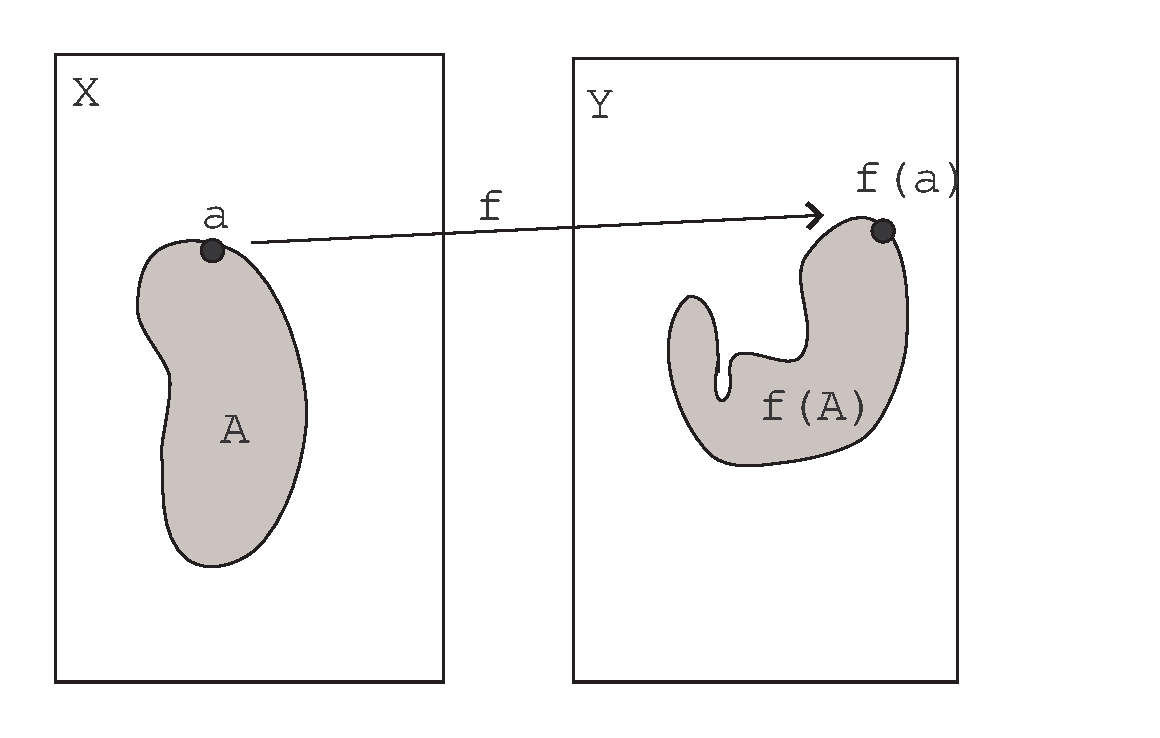
\includegraphics[height=7cm, width=10cm]{fclausu.eps}
    \caption{Interpretaci\'on del inciso d) del Teorema
    \ref{teo,caraccont}}\label{fig,interpretacionteo}
\end{center}
\end{figure}

Ahora veamos que la composici\'on de funciones continuas es
continua.

\begin{proposicion} Sean $(X,d)$, $(Y,d')$, $(Z,d'')$ tres e.m.,
$f:X\rightarrow Y$ y $g:Y\rightarrow Z$ funciones tales que $f$ es
continua en $a\in X$ y $g$ es continua en $f(a)\in Y$. Entonces
$g\circ f:X\rightarrow Z$ es continua en $a$.
\end{proposicion}
\begin{demo} Sea $W$ un entorno de $g(f(a))$. Como $g$ es continua
en $f(a)$ entonces $V:=g^{-1}(W)$ es un entorno de $f(a)$. Luego,
como $f$ es continua en $a$, $f^{-1}(V)=f^{-1}(g^{-1}(W))$ es un
entorno de $a$. Esto implica la tesis, pues
$f^{-1}(g^{-1}(W))=(g\circ f)^{-1}(W)$.
\end{demo}

\begin{corolario} Sea $f:X\rightarrow Y$ una funci\'on continua
en $a$. Supongamos que $Z\subset X$ es un subespacio con $a\in Z$.
Entonces la restricci\'on de $f$ al subespacio $Z$, con la
m\'etrica de subespacio, es continua en $a$.
\end{corolario}
\begin{demo} La susodicha restricci\'on es la composici\'on de $f$
con la inyecci\'on natural $j:Z\rightarrow X$. Por lo tanto el
resultado sigue del hecho que la composici\'on de funciones
continuas es continua.
\end{demo}

Otro concepto importante es el de funci\'on uniformemente
continua.

\begin{definicion} Sea $f$ una funci\'on entre dos e.m. $(X,d)$ e $(Y,d')$.
Diremos que $f$ es \emph{uniformemente continua} si para todo
$\epsilon>0$ existe un $\delta>0$ tal que
$d'(f(x),f(y))<\epsilon$, si $d(x,y)<\delta$.
\end{definicion}

No es facil entender la diferencia de esta definici\'on con la que
expresa que $f$ es continua en cada punto de $X$. La diferencia es
que el $\delta$ de esta definici\'on es el mismo para todos los
puntos de $X$. Mientras que decir que $f$ es continua en cada
punto de $X$ implicar\'{\i}a, en principio, la existencia de un
delta  que puede depender del punto. Los siguientes ejemplos
aclararan m\'as esta definici\'on.

\begin{ejemplo} Las funciones constantes son uniformemente
continuas. Dado un $\epsilon>0$ podemos tomar cualquier valor de
$\delta$ que seguramente cumplir\'a la definici\'on.
\end{ejemplo}
\begin{ejemplo} Una funci\'on puede ser continua en todo punto y,
sin embargo, no ser uniformemente continua,, como muestra el
siguiente ejemplo: Sea $f:\rr\rightarrow\rr$ definida por
$f(x)=x^2$. Esta $f$ es continua en todo punto y no uniformemente
continua. En efecto, la diferencia $(a+h)^2-a^2=2ah+h^2$ tiende a
$+\infty$ si $a$ tiende a $+\infty$. De modo que asegurar que
$h<\delta$ no implica que las imagenes de $a+h$ y $a$ esten cerca,
no importando, para ello, cuan chico sea $\delta$. Ver Figura
\ref{fig,nouncon}.
\end{ejemplo}
\begin{figure}
\begin{center}
    \psfrag{a}{$a$}
    \psfrag{a+h}{$a+h$}
    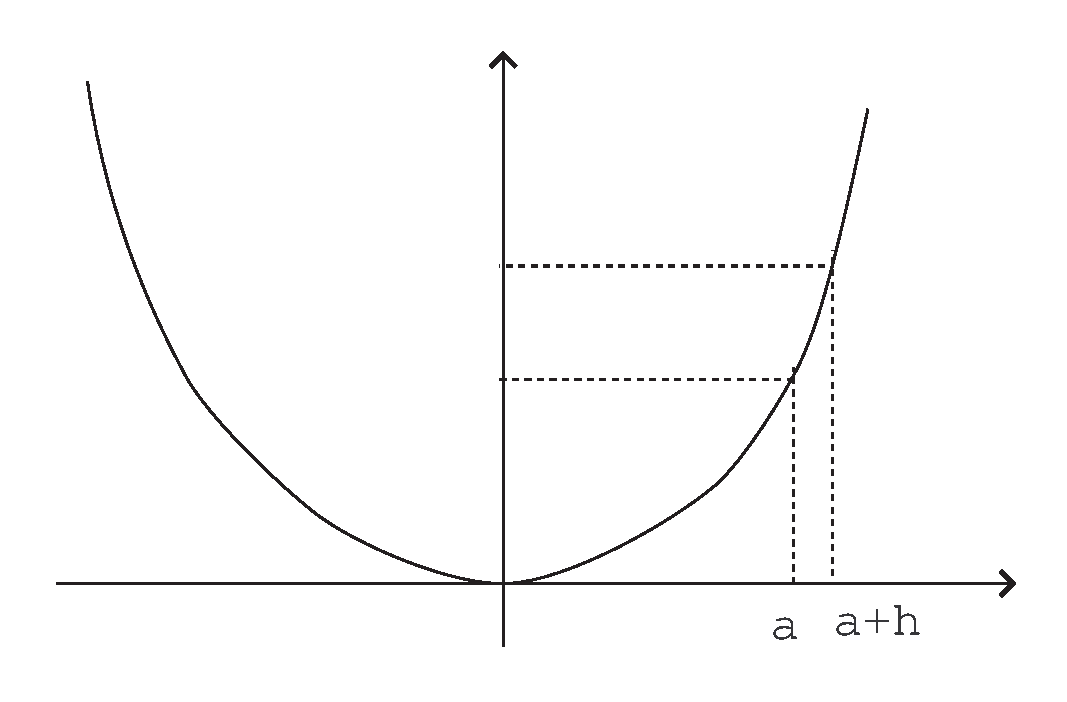
\includegraphics[height=7cm, width=10cm]{nounco.eps}
    \caption{Funci\'on no uniformemente
    continua}\label{fig,nouncon}
\end{center}
\end{figure}

Si una funci\'on es uniformemente continua es continua en cada
punto. La demostraci\'on de este hecho es bastante directa y
simple.
\begin{ejemplo} Sea $(X,d)$ un e.m. y $A\subset X$. La funci\'on:
\[
    \begin{split}
        f:&X\longrightarrow \rr\\
        &x\longmapsto d(x,A).
    \end{split}
\]
es uniformemente continua. Esto es consecuencia de la desigualdad
probada en el Ejercicio \vref{daconjeslipschitz}, a saber:
\[
    |d(x,A)-d(y,A)|\leq d(x,y).
\]
\end{ejemplo}

\section{Homeomorfismos e isometr\'{\i}as}

\begin{definicion} Sean $(X,d)$, $(Y,d')$ dos e.m. y
$f:X\rightarrow Y$ una funci\'on \emph{biyectiva}. Diremos que $f$
es un \emph{homeomorfismo} si $f$ y $f^{-1}$ son ambas continuas.
Dos e.m. tales que exista un homeomorfismo entre ellos se
denominaran homeomorfos.
\end{definicion}

\begin{ejemplo} Dos intervalos abiertos cualesquiera de $\rr$ son
homeomorfos, uno puede construir una funci\'on lineal, que son
homeomorfismos, que aplique uno en el otro. Mientras que un
intervalos abierto  cualquiera $(a,b)$ es homeomorfo a $\rr$. Un
homeomorfismo entre ambos es la funci\'on:
\[
    \begin{split}
        f:&(a,b)\longrightarrow\rr\\
          &x\longmapsto
          \text{tan}\biggl(\pi\frac{2x-(a+b)}{2(b-a)}\biggr)
    \end{split}
\]
\end{ejemplo}

\begin{ejemplo} Un intervalo cerrado ya no es homeomorfo a $\rr$,
esto lo demostraremos m\'as adelante. No obstante podemos definir
la \emph{recta real extendida} que ser\'a homeomorfa a los
intervalos cerrados. M\'as precisamente, sea $f:\rr\rightarrow
(-1,1)$ la funci\'on $f(x)=x/(1+|x|)$. No es dif\'icil demostrar
que $f$ es biyectiva, de hecho analizando esta funci\'on con las
herramientas aprendidas en C\'alculo I vemos que tiene la forma de
la Figura \vref{fig,graffunc}. Definamos el conjunto
$\overline{\rr}$, al que llamaremos \emph{recta extendida}, como
la uni\'on de $\rr$ con dos nuevos elementos, a los que llamaremos
$-\infty$ y $+\infty$. Ahora extendemos $f$ de $\overline{\rr}$ al
$[-1,1]$ por $f(+\infty)=1$ y $f(-\infty)=-1$. Definimos la
funci\'on $d:\overline{\rr}\times\overline{\rr}\rightarrow \rr$
por: \begin{equation}\label{eq,defiso}
    d(x,y)=|f(x)-f(y)|.
\end{equation}
\begin{figure}[h]
\begin{center}
    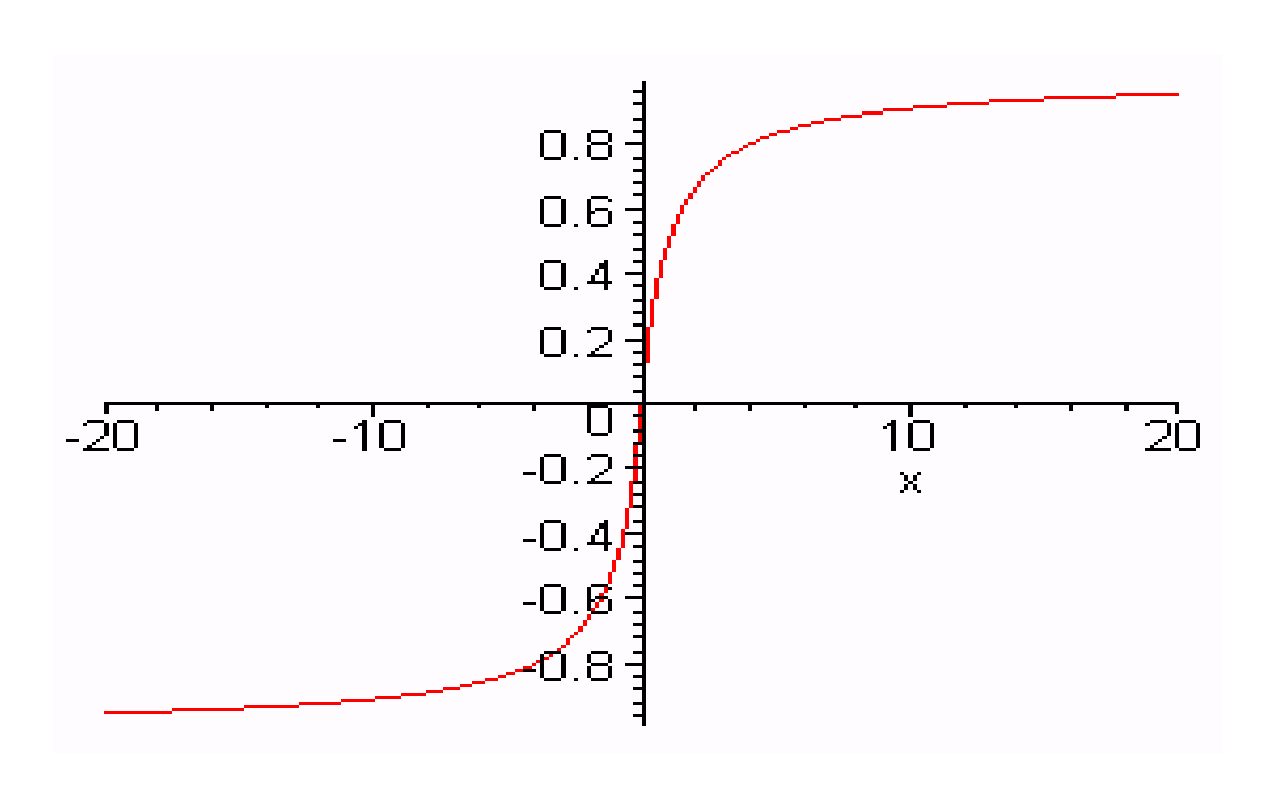
\includegraphics[height=8cm, width=10cm]{graffun.eps}
    \caption{Grafico de la funci\'on $f(x)=x/(1+|x|)$ seg\'un el
    programa  Maple}\label{fig,graffunc}
\end{center}
\end{figure}

La funci\'on $d$ es una m\'etrica en $\overline{\rr}$ (la sencilla
demostraci\'on la desarrollaremos en clase). Con esta m\'etrica el
conjunto $\rr$ es acotado, de hecho $\delta(\rr)=2$. Adem\'as la
funci\'on $f$ resulta un homeomorfismo de $\overline{\rr}$ en
$[-1,1]$ (este \'ultimo con la m\'etrica del m\'odulo). En efecto,
en virtud de la ecuaci\'on \vref{eq,defiso}, dado $\epsilon>0$
basta elegir $\delta=\epsilon$ para verificar que $f$ es
uniformemente continua. Si llamamos $g$ a la inversa de $f$ y
reemplazamos $x$ e $y$ en \vref{eq,defiso} por $g(t)$ y $g(s)$
respectivamente, comprobamos que
\begin{equation}\label{eq,defisoinv}
    d(g(t),g(s))=|t-s|.
\end{equation}
Lo cual implica que $g$ es uniformemente continua, por razones
similares a las que invocamos para $f$. En particular $f$ y su
inversa son continuas, de modo que $f$ es un homeomorfismo.


\end{ejemplo}

En el ejemplo anterior las funciones $f$ y $g$ tienen una
propiedad m\'as fuerte que la de ser homeomorfismos, esta
propiedad la definimos a continuaci\'on.
\begin{definicion} Sean $(X,d)$, $(Y,d')$ dos e.m. y
$f:X\rightarrow Y$ una funci\'on biyectiva. Se dir\'a que $f$ es
una \emph{isometr\'{\i}a} si para todos $x$ e $y$ en $X$ se tiene
que:
\[
    d'(f(x),f(y))=d(x,y).
\]
Si, entre dos e.m. existe una isometr\'{\i}a diremos que los
espacios son \emph{isom\'etricos}.
\end{definicion}

Una isometr\'{\i}a es un homeomorfismo, la idea central de la
demostraci\'on de esta afirmaci\'on est\'a en el ejemplo anterior.
Igual que en aquel ejemplo, hay que demostrar que la inversa de
una isometr\'{\i}a es, a la vez, una isometr\'{\i}a.

\begin{proposicion} Sean $(X,d)$, $(Y,d')$ dos e.m. y
$f:X\rightarrow Y$ una funci\'on biyectiva con inversa $g$.
Entonces son equivalentes:
\begin{itemize}
\item[i)] $f$ es un homeomorfismo.
\item[ii)] $A\subset X$ es abierto si, y solo si, $f(A)$ es
abierto.
\end{itemize}
\end{proposicion}
\begin{demo} i)$\Rightarrow$ii). Sea $A\subset X$. Supongamos, en primer lugar,
que $A$ es abierto. Como $g:Y\rightarrow X$ es continua,
$g^{-1}(A)=f(A)$ es abierto. Supongamos, ahora, que $f(A)$ es
abierto. Como $f$ es continua, $f^{-1}(f(A))=g(f(A))=A$ es
abierto. Esto concluye la demostraci\'on de la primera
implicaci\'on.

ii)$\Rightarrow$i). Tenemos que demostrar que $f$ y $g$ son
continuas. Veamos, primero, que $f$ es continua. Sea $B$ un
abierto de $Y$, hay que demostrar que $f^{-1}(B)=g(B)$ es un
abierto de $X$. Pero $B=f(g(B))$ y $B$ es abierto, entonces, por
ii), $g(B)$ es abierto. Veamos, ahora, que $g$ es continua. Sea
$A$ abierto en $X$. Luego, por ii), $g^{-1}(A)=f(A)$ es abierto en
$Y$, por lo cual, $g$ es continua.
\end{demo}

Este teorema nos dice que si dos espacios son homeomorfos,
entonces existe una correspondencia de los abiertos de uno con los
del otro espacio.

El conjunto formado por todos los conjuntos abiertos, se denomina
\emph{topolog\'{\i}a}. Brevemente, digamos que un \emph{espacio
topol\'ogico} es un par $(X,\tau)$, donde $\tau\subset
\mathcal{P}(X)$\footnote{$\mathcal{P}(X)$ es el conjunto de partes
de $X$, es decir $\tau$ es un conjunto cuyos elementos son
subconjuntos de $X$}, que satisface los siguientes axiomas:
\begin{itemize}
    \item[1)] $\emptyset, X\in \tau$
    \item[2)] Si $G_i\in\tau$, para $i\in I$, entonces
    $\bigcup_{i\in I}G_i\in \tau$.
    \item[3)] Si $G_i\in\tau$, para $i\in I$, e $I$ es finito, entonces
    $\bigcap_{i\in I}G_i\in \tau$.
\end{itemize}

En un espacio topol\'ogico uno puede construir la nociones, que
hemos construido para e.m., por ejemplo conjunto cerrado,
interior, clausura,  entorno, funci\'on continua y espacio
separable. Por tanto, estas propiedades se denominan
topol\'ogicas. Las propiedades topol\'ogicas son invariantes por
homeomorfismos, por ejemplo si un espacio es separable, cualquier
homeomorfo a \'el tambi\'en lo es. Algunas propiedades no son
topol\'ogicas, por ejemplo que una funci\'on sea uniformemente
continua, puesto que para definir este concepto necesitamos de una
m\'etrica.

Un mismo conjunto $X$, puede tener dos m\'etricas distintas, por
ejemplo en $\rr$ tenemos la m\'etrica euclidea y la discreta.
Podemos plantearnos que estas m\'etricas den origen a una misma
topolog\'{\i}a, si esto sucede diremos que las dos
\emph{m\'etricas son equivalentes}.


\section{Ejercicios}

\begin{ejercicio} Sea $(X,d)$ un e.m. y $A\subset X$. Demostrar
que $A\cup \text{Ext}(A)$ es denso en $A$. ?`Ser\'a cierto que
$A^0\cup \text{Ext}(A)$ es, siempre, denso?
\end{ejercicio}

\begin{ejercicio} Demostrar que $\mathbb{I}:=\rr-\mathbb{Q}$ es
separable. Exhibir un conjunto denso numerable.
\end{ejercicio}

\begin{ejercicio} Sea $A\subset \rr$. Definamos $B:=\{x\in
A|\exists y>x: (x,y)\cap A=\emptyset\}$. Demostrar que $B$ es a lo
sumo numerable.
\end{ejercicio}

\begin{ejercicio} Sea $(X,d)$ un e.m. y $A\subset X$. Diremos que
$a\in A$ es un \emph{punto aislado} de $A$ si existe un entorno
$U$ de $a$ tal que $U\cap A=\{a\}$. En la Figura
\vref{fig,aislado} el conjunto $A$ consiste de la parte sombreada
y el punto $a$, este \'ultimo es un punto aislado, pues el entorno
$U$ satisface la definici\'on.

\begin{figure}[h]
\begin{center}
    \psfrag{A}{$A$}
    \psfrag{U}{$U$}
    \psfrag{a}{$a$}
    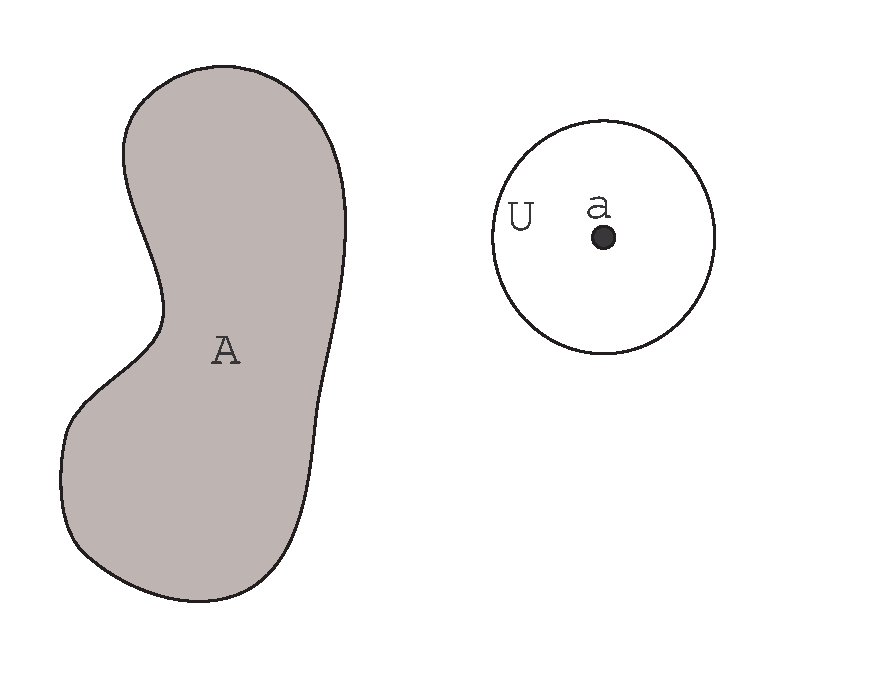
\includegraphics[height=5cm, width=10cm]{aislado.eps}
    \caption{Punto aislado}\label{fig,aislado}
\end{center}
\end{figure}


Por otra parte, un punto $a\in X$ es un \emph{punto de
acumulaci\'on} de $A$ si, para todo entorno $U$ de $a$ se tiene
que $(U-\{a\})\cap A\neq\emptyset$.

Sea $A$ un conjunto, $B$ el conjunto de puntos de acumulaci\'on de
$A$ y $C$ el conjunto de puntos aislados de $A$. Demostrar los
siguientes items:
\begin{itemize}
    \item[a)] $B$ es cerrado, y $\overline{A}=B\cup C$.
    \item[b)] Si $X$ es separable entonces $C$ es numerable.
\end{itemize}
\end{ejercicio}

\begin{ejercicio} Demostrar que $(X,d)$ es separable si y solo si
 todo cubrimiento de $X$ por abiertos\footnote{Un cubrimiento por
abiertos de $X$ es una familia de conjuntos abiertos
$\{G_i\}_{i\in I}$ tal que $X=\bigcup_{i\in I}G_i$.} tiene un
subcubrimiento a lo sumo numerable\footnote{Es decir existe una
subfamilia a lo sumo numerable de la familia $\{G_i\}$ que
tambi\'en es un cubrimiento.}. \emph{Ayuda:} Sea $\{U_i\}_{i\in
I}$ un cubrimiento de $X$ y $\{G_n\}_{n\in\nn}$ una base
numerable. Para cada $n\in\nn$ elegir un $i_n$ tal que $G_n\subset
U_{i_n}$. Luego la familia $\{U_{i_n}\}_{n\in\nn}$ ser\'a un
cubrimiento.
\end{ejercicio}

\begin{ejercicio} Sea $(X,d)$ un e.m., $A\subset X$ y $B\subset
A$.  Demostrar que $B^0\subset B^0_A$. Dar un ejemplo donde
$B^0\neq B^0_A$.
\end{ejercicio}

\begin{ejercicio} Sea $(X,d)$ un e.m., $B$ y $C$ subconjuntos de
$X$ y $A\subset C\cap B$. Demostrar que $A$ es abierto (cerrado)
en $B\cup C$ si, y solo si, es abierto (respectivamente cerrado)
en $B$ y $C$.
\end{ejercicio}

\begin{ejercicio} Sea $\{G_i\}_{i\in I}$ un cubrimiento por abiertos de un e.m.
$X$. Demostrar que $F\subset X$ es cerrado si, y solo si, $F\cap
G_i$ es cerrado para todo $i\in I$.
\end{ejercicio}

\begin{ejercicio} Dar un ejemplo de un subespacio $A$ de $\rr^2$
tal que exista una bola abierta que es un conjunto cerrado, pero
no una bola cerrada, y una bola cerrada que es un conjunto
abierto, pero no una bola abierta. Ayuda: Considerar $A$ formado
por los puntos $(0,1)$, $(0,-1)$ y por un subconjunto apropiado
del eje $x$.
\end{ejercicio}


\begin{ejercicio} Sean $(X,d)$, $(Y,d')$ e.m., $A$ y $B$
subconjuntos de $X$ tales que $A\cup B=X$.
\begin{itemize}
\item[i)] Sea $f:X\rightarrow Y$ una funci\'on tal que
$f_{|A}$\footnote{$f_{|A}$denota la restricci\'on de $f$ al
conjunto $A$} y $f_{|B}$ son ambas continuas en $x\in A\cap B$,
probar que $f$ es continua en $x$.
\item[ii)] Dar un ejemplo de funci\'on tal que $f_{|A}$, $f_{|B}$ y $f_{|A\cap
B}$sean continuas pero $f$ no lo sea.
\end{itemize}
\end{ejercicio}

\begin{ejercicio} Sean $(X,d)$, $(Y,d')$ e.m. y $f:X\rightarrow Y$
una funci\'on. Demostrar que son equivalentes:
\begin{itemize}
\item[i)] $f$ es continua.
\item[ii)] Para todo $B\subset Y$: $f^{-1}(B^0)\subset
\bigl[f^{-1}(B)\bigr]^0$.
\item[iii)]Para todo $B\subset Y$: $\overline{f^{-1}(B)}\subset
f^{-1}(\overline{B})$.
\end{itemize}
Dar un ejemplo de funci\'on continua donde
$\overline{f^{-1}(B)}\neq f^{-1}(\overline{B})$.
\end{ejercicio}

\begin{ejercicio} Sean $(X,d)$, $(Y,d')$ e.m. y $f,g:X\rightarrow Y$
 funciones continuas. Demostrar que:
 \begin{itemize}
    \item[i)]  El conjunto $\{x\in X| f(x)=g(x)\}$ es cerrado.
    \item[ii)] Si $f$ y $g$ coinciden en un conjunto denso
    entonces son iguales.
 \end{itemize}
 \end{ejercicio}

\begin{ejercicio} Sean $(X,d)$, $(Y,d')$ e.m.. Demostrar que son equivalentes
\begin{itemize}
    \item[i)] Toda funci\'on $f:X\rightarrow Y$ es continua.
    \item[ii)] Todo punto de $X$ es aislado\footnote{Por abuso de
    lenguaje los e.m. con esta propiedad se denominan discretos}.
\end{itemize}
\end{ejercicio}


\begin{ejercicio} Sean $(X,d)$, $(Y,d')$ e.m. y $f:X\rightarrow Y$
 una funci\'on biyectiva. Demostrar que $f$ es un homeomorfismo
 si, y solo si, para todo $A\subset X$ tenemos que
 $f(\overline{A})=\overline{f(A)}$.
 \end{ejercicio}

 \begin{ejercicio} Demostrar:
 \begin{itemize}
    \item[i)] que las m\'etricas sobre $\rr^n$
    definidas en los Ejemplos \vref{ejem,disteuclidea},
    \vref{ejem,distl1} y \vref{ejem,distlinf} son todas equivalentes.
    \item[ii)] que las distancias $d$ , $d_1$ y $d_2$ del Ejercicio
    \vref{ejer,distequiv} son equivalentes.
    \item[iii)] Dados dos topolog\'{\i}as $\tau_1$ y $\tau_2$
    sobre el mismo espacio $X$ decimos que $\tau_1$ es m\'as fina
    que $\tau_2$ si $\tau_2\subset \tau_1$. Demostrar que, sobre $C([0,1])$,
    la topolog\'{\i}a que genera la m\'etrica del
    Ejemplo \vref{ejem,distsobrecont} es m\'as fina que la
    topolog\'{\i}a que genera la m\'etrica del Ejemplo
    \vref{ejem,distsobrecont} es m\'as fina que la del
    Ejemplo \vref{ejem,distsobrecontl1}.
 \end{itemize}
 \end{ejercicio}
